% IGARSS 2027 paper skeleton (12 Oct 2026).
% Uses IEEEtran (conference) as a stand-in until the official IGARSS 2027
% author kit is posted (portal opens 10 Nov 2026); the section files in
% sections/ move over unchanged. 4 pages including references, as in older
% IGARSS kits (check the 2027 rule).
% Compile:  tectonic main.tex
% AI assistance: Claude (Anthropic) set up this skeleton, the tables and the
% figures, and drafted Data and Methods (13 Oct) and the Introduction,
% Results, Discussion and abstract (21 Oct) for Brian to rewrite. Disclose
% as IGARSS and CSE 5999 require.
\documentclass[conference]{IEEEtran}
\usepackage[T1]{fontenc}   % Times with bold under XeTeX (tectonic)
\usepackage{graphicx}
\usepackage{amsmath}
\usepackage{booktabs}
\usepackage{xcolor}
\usepackage{cite}
\usepackage[hidelinks]{hyperref}
\graphicspath{{figures/}{../travel-speed-gate1/results/t4_terrain_curve/}{../travel-speed-gate1/results/t4_trail_map/}{../travel-speed-gate1/results/t4_mode_curves/}}
\newcommand{\todo}[1]{\textcolor{red}{[TODO: #1]}}

\begin{document}

\title{Does Remote Sensing Beat the Trail Map? Predicting Hiking Speed in
Unseen Regions from Lidar Terrain and OpenStreetMap Tags}

\author{\IEEEauthorblockN{Brian Zhou \todo{author list and order: ask
Danni, Tianyi and Prof.\ Jacobs}}
\IEEEauthorblockA{Department of Computer Science and Engineering,
Washington University in St.\ Louis}}

\maketitle

\begin{abstract}
% DRAFT by Claude (21 Oct 2026), summarizing the drafted sections. Brian:
% rewrite it in your own words (~145 words now; keep it short for 4
% pages) and disclose the AI assistance.
\todo{Draft by Claude: rewrite in your own words.}
Estimates of walking time on trails still rely on Tobler's 1993 hiking
function. We ask what corrects it in regions a model has never seen, using
290,640 walking traversals of 50~m trail segments from public
OpenStreetMap (OSM) GPS traces in 17 North American mountain regions.
Holding out one region at a time and scoring calibrated predictive
distributions (CRPS), we find Tobler's function 12.5\% worse than a
refitted slope curve. Terrain from elevation models, mostly airborne
lidar, improves CRPS by 2.1--2.8\% in unseen regions and beats OSM trail
tags in 16 of 17; tags add 0.4--0.9\%, and lidar vegetation and satellite
embeddings help mainly where the model was trained. For the same hiker on
the same trail, descending is 8--23\% faster than climbing, not 42\% as
Tobler implies. A one-input terrain-adjusted Tobler function keeps part of
the gain, but a hiker's own pace still matters most over whole hikes.
\end{abstract}

\begin{IEEEkeywords}
hiking speed, lidar, OpenStreetMap, GPS trajectories, transfer, calibration
\end{IEEEkeywords}

\section{Introduction}
\label{sec:intro}

% ~0.5 page. Notes from OUTLINE.md; turn them into prose.
\todo{Paragraph 1, why travel time on foot matters: search and rescue,
wildfire escape routes, trail apps, accessibility maps. GIS still uses
Tobler's 1993 hiking function~\cite{tobler1993},
$v = 6\exp(-3.5\,|s + 0.05|)$ km/h, and fixed multipliers for other
modes.}

\todo{Paragraph 2, what is known: crowdsourced GPS shows Tobler is too fast
and too peaked~\cite{campbell2019crowdsourced,campbell2022variability};
Wood et al.~\cite{wood2023hiking} add OSM terrain classes and lidar
obstruction (England and Wales); Huang et al.~\cite{huang2026modeling} fit
boosted trees with 16 factors, weather included (Hong Kong); \v{S}eri\'c et
al.~\cite{seric2022modeling} predict a latent walking speed from Sentinel-2
(one Croatian range); HikingTTE~\cite{asako2024hikingtte} learns whole-hike
time from the hiker's first part. STRIDE~\cite{campbell2024stride} models
walking speed from lidar slope, understory
density~\cite{campbell2018understory} and roughness, calibrated on field
walks; RasterNet~\cite{hadzic2020rasternet} learns road speed from lidar
and imagery.}

\todo{Paragraph 3, the gap: each of these studies fits and tests in one
country, city or range with random or within-area splits (Wood: 10-fold
cross-validation; Huang: random split); none tests whether terrain
covariates transfer to regions a model has never seen, against the map tags
used today, with calibrated uncertainty. Wood et al. also found no gain over
existing functions for whole-route times (13.5--15.5\% error for every
model).}

\todo{Paragraph 4, contributions (three bullets): (1) a 17-region dataset of
walking traversals of 50~m trail segments from public OSM traces; (2) an
evaluation protocol (leave one region out, CRPS, coverage) with published
baselines; (3) the finding that elevation-derived terrain transfers and map
tags do not, plus a one-input terrain-adjusted hiking function.}

\section{Data}
\label{sec:data}

% DRAFT by Claude (13 Oct 2026), written from the pipeline code and the
% final results (docs/NEXT_STEPS.md section 1a; results/t1_all/DATA_CARD.md).
% Brian: rewrite it in your own words, and disclose the AI assistance
% (CSE 5999 and IEEE both require it).
\todo{Draft by Claude: rewrite in your own words.}

\textbf{Sources.} We use public GPS traces uploaded to
OpenStreetMap (OSM)~\cite{osm} in 17 mountain regions of the United States
and Canada (Fig.~\ref{fig:map}), chosen for relief, trail density and lidar
coverage. The traces come from three sources: the OSM trackpoints API,
which returns the timestamped points of identifiable and trackable uploads
tile by tile; the original GPX files of identifiable uploads, which give
whole hikes at the device's own sampling; and a crawl of 1.5 million
original files of public and identifiable uploads from 2016--2022, which
keeps the timestamps the API drops. Sixteen regions combine all three; the
Bay Area uses the crawl only, because the API times out on its tiles.

\textbf{Processing.} Each recording is cleaned (repeated timestamps,
steps faster than 60~km/h), split at gaps over 5~min and thinned to points
at least 5~s apart. A step counts as a stop when the point 60~s later lies
within 10~m. Traces are map-matched to the OSM trail and road network with
a hidden Markov model~\cite{newson2009hidden} (97\% of points matched), and
the matched path is cut into 50~m segments. Each segment records its moving
speed, its signed slope along the direction of travel from the 5~m USGS
3DEP elevation grid~\cite{sugarbaker2017status} (resampled from 1~m lidar
under at least 83\% of walked trail in 13 regions), the OSM tags of its way
and the trace's recording interval. Duplicate uploads are removed, and
traces that start within 15~min and 1~km of each other form one outing (a
group hike), the unit we resample. Travel mode is inferred per trace,
anchored on trails closed to bikes and horses. Against the activity that
327 uploaders' apps wrote into their files, 93\% of labelled hikes are
classed as walking, and 5\% of the labelled traces we class as walking say
bike or ski.

\textbf{The dataset.} The regions hold 2,876 hiking traces. The walking
analysis set (walking traces on trails) has 290,640 segments (14,532~km)
from 2,046 traces in 1,992 outings and 4,702 moving hours. Its uploaders are
OSM mappers and enthusiasts rather than a random sample of hikers, and busy
API tiles do not reach their oldest uploads. Traces logged more than 10~s
apart read up to 11\% slow, because straight lines between points cut
corners and short stops hide between them; the gains we report are the
same at every recording rate (Sec.~\ref{sec:results}).

\begin{figure}[t]
\centering
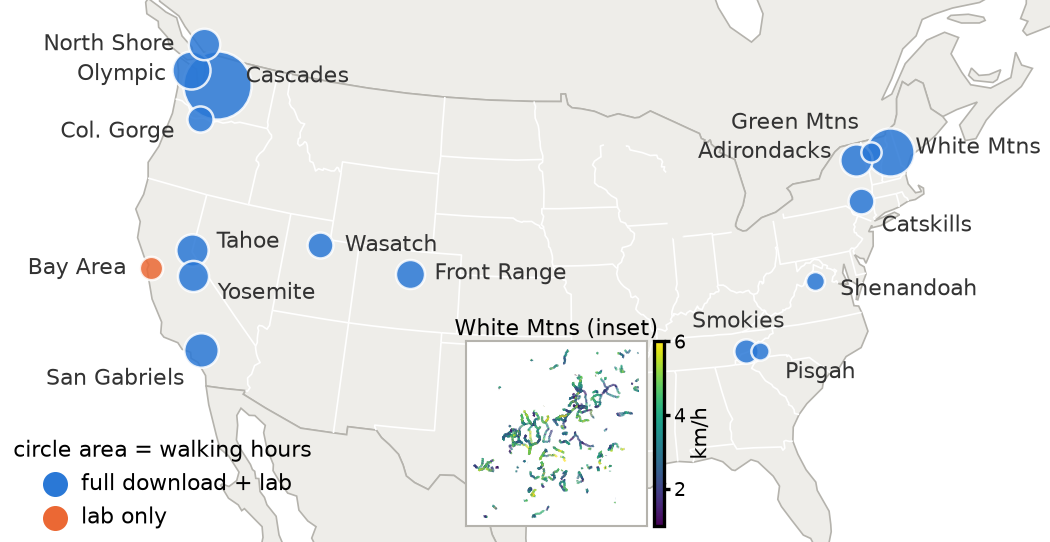
\includegraphics[width=\columnwidth]{fig_map}
\caption{The 17 regions. Circle area is walking hours (1,992 outings,
4,702 h in total). Blue: full OSM download plus the lab crawl; orange: lab
crawl only. Inset: the White Mountains' 34,535 walking segments colored by
speed.}
\label{fig:map}
\end{figure}

\section{Methods}
\label{sec:methods}

% ~0.75 page. Code: travel-speed-gate1/t3_harness.py, t2_terrain5m.py,
% t2_terrain1m.py, t2_embed.py, t4_terrain_curve.py.
\todo{Target: the distribution of $\ln v$ for a walking trail segment.}

\todo{Covariates. (a) Slope. (b) OSM tags: sac\_scale, trail\_visibility,
surface, width, smoothness, mtb\_scale, highway, access. (c) Terrain from
elevation, read every 1~m along the segment's matched path: spread and
maximum of 5~m pitches, relief along the line of travel, side slope (5~m
grids; 1~m lidar adds STRIDE's roughness). (d) NLCD 30~m canopy and land
cover. (e) AlphaEarth satellite embeddings~\cite{alphaearth2025}.
Control: ``hidden climbing'', the extra time a fixed Tobler curve predicts
when the segment is walked as 5~m pieces.}

\todo{Models: published Tobler, Campbell (median)~\cite{campbell2022variability}
and STRIDE~\cite{campbell2024stride}; a refitted rounded asymmetric slope
curve (the baseline); additive ridge offsets on binned features; gradient
boosted trees.}

\todo{Predictive distribution: prediction plus residual quantiles from held
out training outings, so calibration has to transfer too.}

\todo{Splits (never by segment): 5 folds of outings; 5 folds of 10~km
blocks; leave one region out (17 folds). Score: CRPS~\cite{gneiting2007strictly}
as skill vs the slope curve, 95\% intervals resampling whole regions;
coverage of 90\% intervals; moving-time error per hike. References: the
hiker's pace from their first km; each region's own offset.}

\begin{equation}
\ln v = a_0 + a_1 z - (k_0 + k_1 z)\,|s + s_0|
\label{eq:terrain}
\end{equation}
with $z$ the SD of 5~m pitches along the path divided by 0.10.
\todo{Introduce Eq.~\eqref{eq:terrain}, the terrain-adjusted hiking
function: Tobler's form, with peak speed and slope sensitivity depending on
one DEM-derived number.}

\section{Results}
\label{sec:results}

% DRAFT by Claude (21 Oct 2026), written from the notes that were here and
% the final numbers (docs/NEXT_STEPS.md section 1a; DECISIONS_LOG.md
% #95-#112; results/t3_harness_*/, results/t1_findings/). Brian: rewrite it
% in your own words, and disclose the AI assistance (CSE 5999 and IEEE both
% require it). "a / b" pairs are additive / tree models, as in Table I.
\begin{table}[t]
\centering
\caption{CRPS skill (\%) vs the refitted slope curve: additive / trees;
STRIDE as published (refitted).}
\label{tab:skill}
\footnotesize
\setlength{\tabcolsep}{2.5pt}
\begin{tabular}{@{}lccc@{}}
\toprule
Model & New hikes & New 10 km & \textbf{Unseen region} \\
\midrule
Tobler 1993 & $-12.8$ & $-12.7$ & $-12.5$ \\
Campbell 2022 & $-0.9$ & $-0.9$ & $-0.5$ \\
STRIDE 2024 & $-17.2$ ($+0.2$) & $-17.3$ ($+0.2$) & $-16.8$ ($+0.2$) \\
OSM tags & $+1.3$ / $+1.5$ & $+1.1$ / $+1.5$ & $+0.9$ / $+0.4$ \\
30 m vegetation & $+0.0$ / $+0.1$ & $-0.0$ / $-0.1$ & $-0.1$ / $-0.8$ \\
Embeddings & $+1.4$ / $+2.6$ & $+1.4$ / $+1.9$ & $+1.1$ / $+1.1$ \\
Lidar vegetation$^\dagger$ & $+0.4$ / $+0.5$ & $+0.4$ / $+0.3$ & $+0.3$ / $+0.2$ \\
\textbf{Terrain} & $+2.2$ / $+3.2$ & $+2.1$ / $+2.8$ & $\mathbf{+2.1}$ / $\mathbf{+2.8}$ \\
Terrain + emb.\ + tags & $+3.7$ / $+5.1$ & $+3.8$ / $+5.1$ & $+3.0$ / $+3.9$ \\
Eq.~(1), one input & $+1.0$ & $+1.0$ & $+1.0$ \\
\bottomrule
\end{tabular}\\[2pt]
{\scriptsize $^\dagger$The 15 regions with lidar point clouds.}
\end{table}


\textbf{Tobler's function fails everywhere.} Walking speed peaks near
4.2~km/h on level to gently descending trail, not at 6~km/h
(Fig.~\ref{fig:curve}a): Tobler's function is about 20\% too fast within
$\pm$10\% grade and 18\% too slow on climbs steeper than 25\%, and in
unseen regions it scores $-12.5\%$ (Table~\ref{tab:skill}), worse in all
17. Campbell et al.'s published median curve~\cite{campbell2022variability}
is about 20\% too fast on climbs steeper than 25\%; it ties our refit on
average ($-0.5\%$) but ranges by region from $-3.8\%$ (White Mountains) to
$+5.8\%$ (Shenandoah). Pooled over unseen regions, every model's 90\%
intervals cover about 89\% of segments (as little as 81\% in the North
Shore).

\textbf{Downhill is faster, but less than Tobler implies.} For the same
hiker on the same trail (2,763 out-and-back pairs from 1,145 outings;
Fig.~\ref{fig:curve}b), descending is 8\% faster than climbing at
3--10\% grade and 22--23\% above 20\%, not the 42\% Tobler implies. Our
pooled curve implies nearly the same ratios, so its asymmetry is not an
artifact of who walks which slopes.

\textbf{Map tags transfer less well.} OSM tags improve on the slope curve
for new hikes in known regions ($+1.3\%$ / $+1.5\%$, additive / trees). In
unseen regions the additive model keeps two thirds of that ($+0.9\%$
[0.1, 1.7]) and the trees lose most of it ($+0.4\%$ [$-1.1$, 1.6]).

\textbf{Terrain transfers.} Terrain from elevation gains nearly as much in
unseen regions as within them, $+2.1\%$ [1.5, 3.1] / $+2.8\%$ [1.8, 4.1]. It
beats tags in 16 of 17 held-out regions (Fig.~\ref{fig:skill}b; 14 of 17
with trees) and, on average, even a slope curve refitted on the held-out
region's own other hikers ($+1.2\%$). Terrain minus tags is $+0.7$ to
$+2.2$ points (95\% interval), above zero in every bootstrap draw. Uneven
grade inside the segment, which one average slope hides, carries over half
of the gain: the hidden-climbing control alone gives $+1.2\%$ / $+1.6\%$.
Terrain is neither a region
proxy (within regions it adds $\sim$1.9 points to a learned offset per
region) nor a hiker proxy (it adds $\sim$2.3 points to the hiker's own
pace).

No other input transfers as well. 30~m land cover and canopy add nothing.
AlphaEarth embeddings help within regions ($+1.4\%$ / $+2.6\%$) but less,
and less reliably, in unseen ones ($+1.1\%$). Vegetation from the lidar
point clouds adds at most $+0.2$ points to terrain, within or across the
15 regions. Terrain + tags gives $+2.6\%$ / $+3.0\%$ in unseen regions
(Fig.~\ref{fig:skill}a).
Published STRIDE~\cite{campbell2024stride} scores $-16.8\%$; refitted,
$+0.2\%$.

\textbf{Robustness.} The terrain gain holds for newer hikes (trained to
2019, tested on 2020 on: $+2.2\%$ / $+2.9\%$; tags $+0.9\%$), at
every GPS recording rate ($+1.7\%$ to $+2.4\%$ in unseen regions,
additive) and with no
neighbouring region in training: with a whole zone held out, $+1.9\%$ /
$+2.7\%$ (tags $+0.7\%$ / $-0.1\%$); from West to East and back, $+2.6\%$
/ $+3.3\%$ (tags $+1.5\%$ / $-0.3\%$). It also holds for hikers the
model never saw: holding out uploaders instead of outings changes little
($+2.2\%$ / $+3.2\%$), and leaving out a region together with everyone
who hiked there (0.1--8.5\% of the training data) gives $+1.8\%$ /
$+2.4\%$ (tags $+0.5\%$ / $-0.4\%$), above tags in every draw.

\textbf{Whole hikes: the hiker dominates.} Over 1,354 hike traces in held-out
regions, the median error in moving time after the first kilometre is
13.6\% for the slope curve and 13.0\% with terrain, but 10.0\% with the
hiker's pace on that kilometre and 9.6\% with both.

\begin{figure}[t]
\centering
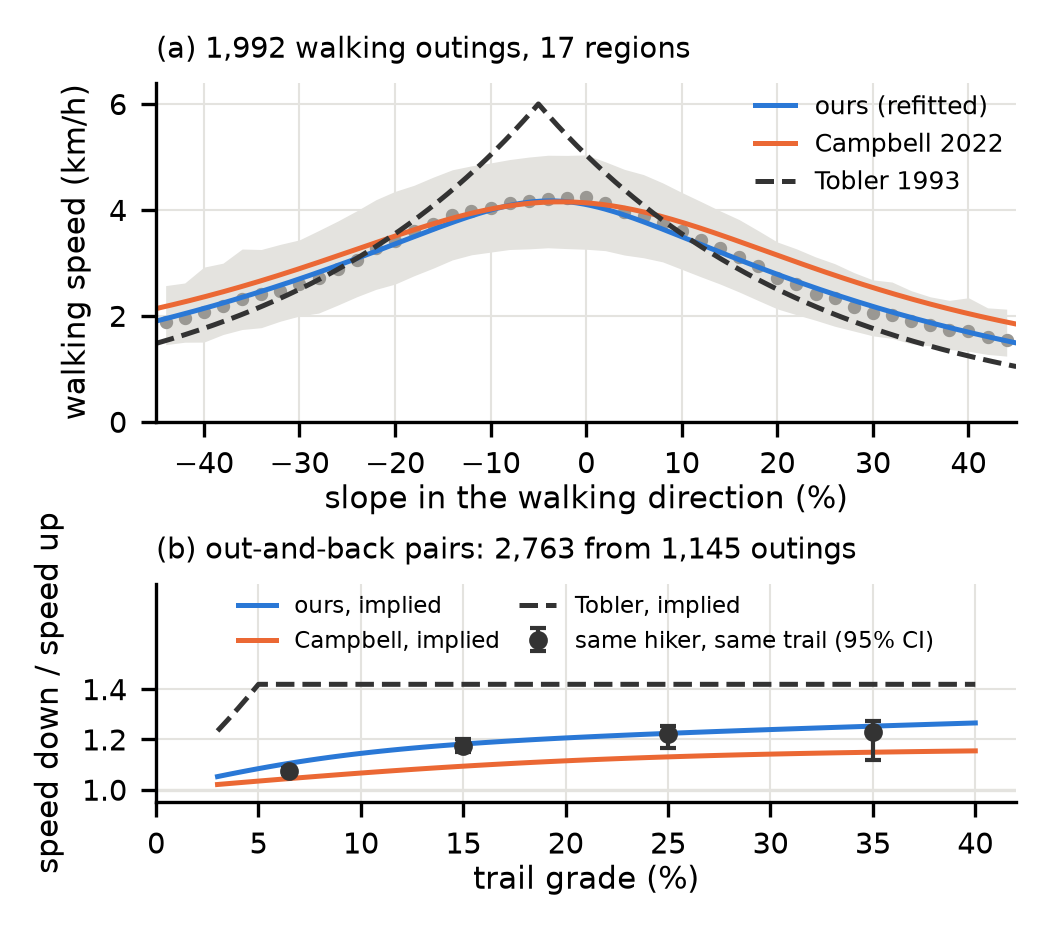
\includegraphics[width=\columnwidth]{fig_curve}
\caption{(a) Walking speed vs slope in the walking direction: median per
2\% bin (dots), middle 50\% of segments (gray), our refitted curve,
Campbell et al.'s median curve~\cite{campbell2022variability} and
Tobler's function~\cite{tobler1993}. (b) Speed down / speed up for the same
hiker on the same trail (out-and-back pairs; 95\% intervals resample
outings) and the ratio each curve implies.}
\label{fig:curve}
\end{figure}

\begin{figure*}[t]
\centering
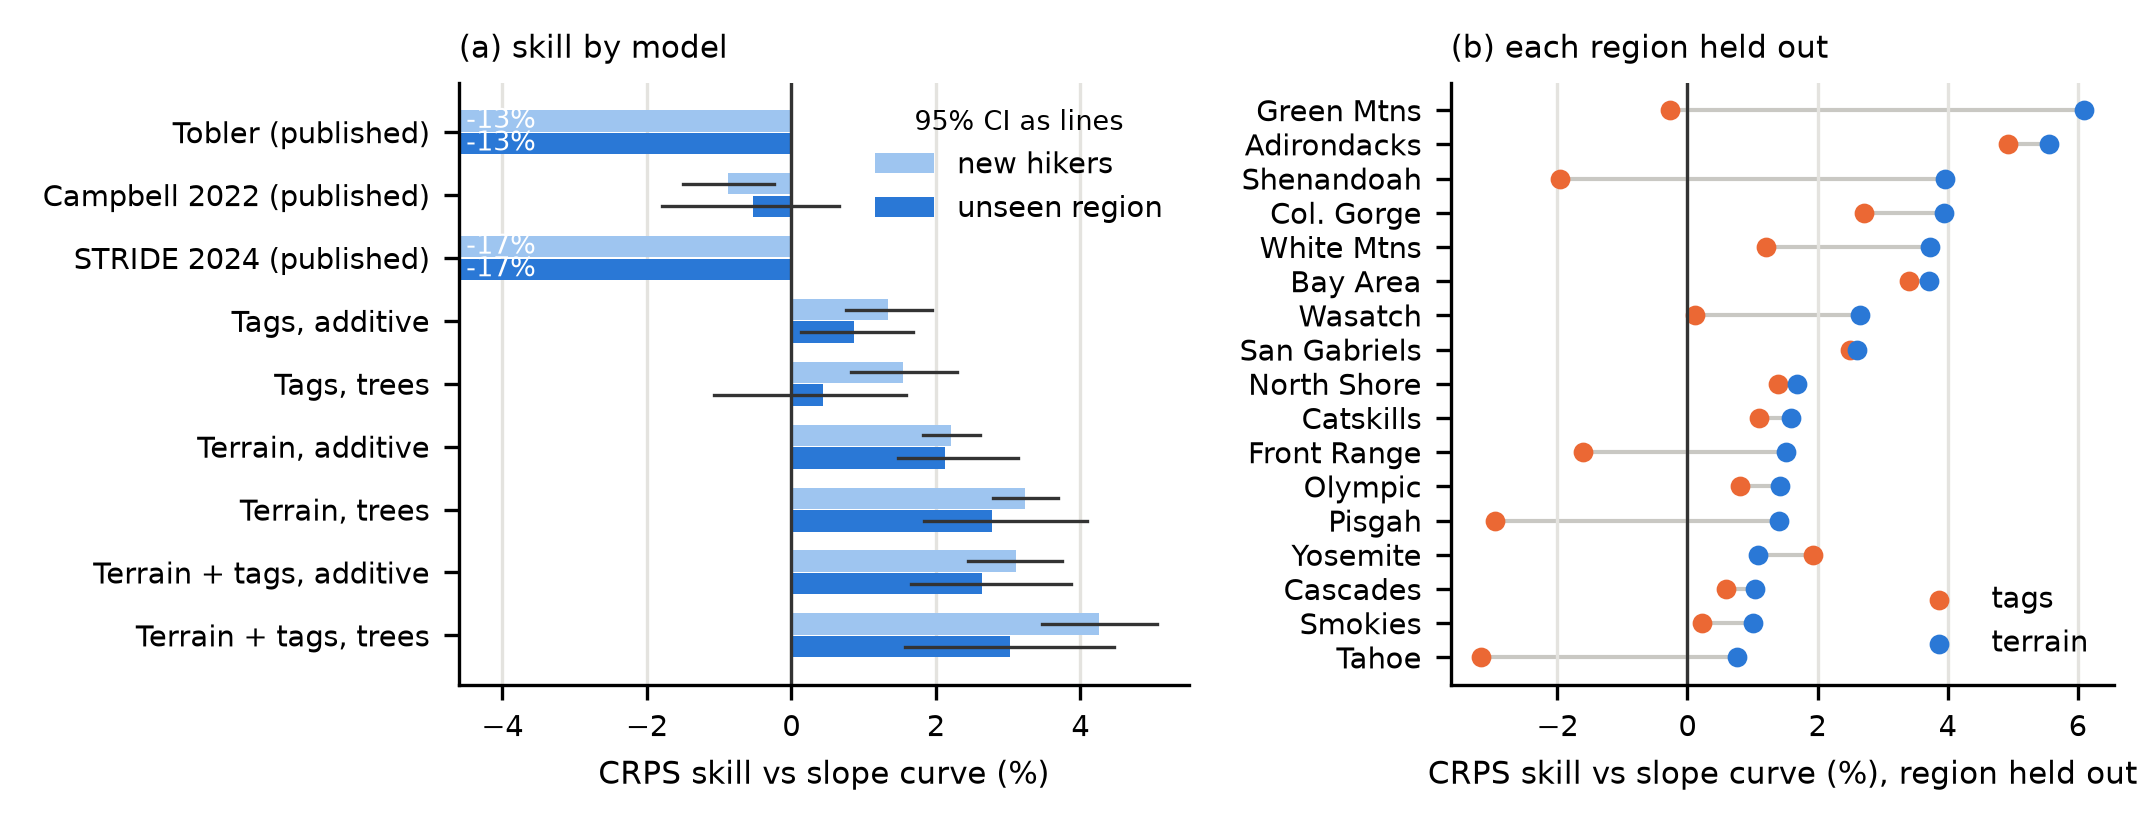
\includegraphics[width=\textwidth]{fig_skill_regions}
\caption{CRPS skill vs the refitted slope curve. (a) By model, for new
hikes in known regions (light; 95\% intervals resample outings) and in
regions the model never saw (dark; intervals resample regions). (b) Each
region held out:
terrain vs OSM tags (additive models); terrain beats tags in 16 of 17.}
\label{fig:skill}
\end{figure*}

% Dropped for the 4-page budget (paper/OUTLINE.md); restore if space allows:
% the travel-mode result (one shared curve x a constant per mode: runners
% x2.5 fine; bikes/skis ~4x walking downhill, ~1.6x uphill, own curve 3.8%
% lower RMSE; DECISIONS_LOG #96, #103);
% fig_hike_time.png (whole-hike time errors, R4) and fig_wm_pace.png (pace on
% every White Mountains trail, the practical output in the Discussion).

\section{Discussion and Conclusion}
\label{sec:discussion}

% DRAFT by Claude (21 Oct 2026), written from the notes that were here and
% DECISIONS_LOG.md (#89, #96, #99, #102, #104-#108, #113). Brian: rewrite
% it in your own words, and disclose the AI assistance.
\todo{Draft by Claude: rewrite in your own words.}

\textbf{Why tags do not transfer.} Not because tag values mean different
things in different places: within the same hike, harder sac\_scale grades
are slower in every region where they are used (mountain\_hiking vs
hiking $-5\%$, 10 of 10 regions; harder grades $-11\%$, 8 of 8). What
varies is where tags exist: sac\_scale is on 1--96\% of walked trail,
depending on the region, and untagged trail is faster than tagged trail in
some regions and slower in others ($-3.5\%$ to $+5.1\%$ within a hike). So
tags inform only part of each region's trails, and boosted trees on tags,
which can fit region-specific tag combinations, lose the most in transfer
($+1.5\% \to +0.4\%$). Terrain exists on every trail, and its effect has
the same sign in all 17 regions (steppiest vs smoothest fifth, $-12\%$).

\textbf{What terrain captures.} Uneven grade within the segment, such as
rock steps and short pitches, plus difficulty beyond grade. Its gain is
largest on descents and level trail ($+2.3$ to $+2.8\%$, additive) and
smallest on steep climbs ($+0.8\%$), consistent with footing setting the
pace going down and effort going up. The signal is the trail's elevation
profile, not micro-relief: 1~m lidar adds little over the 5~m grid, and
STRIDE's off-path roughness and understory terms add nothing on trails or
make it worse ($-18\% \to -35\%$).

\textbf{Use.} Eq.~(\ref{eq:terrain}) needs only a DEM. Fitted on the other
16 regions, it gives a pace for all 3,369~km of White Mountains trail,
77\% of which no trace in our data covers (median 15.2~min/km, vs 12.8 for
Tobler). It travels less far than the full terrain model, though
($+0.6\%$ with a whole zone held out, $-0.3\%$ between East and West).

\textbf{Limits.} Our hikers are OSM uploaders, not a random sample. Sparse
traces read slow (Sec.~\ref{sec:data}); hiking functions depend on the
sampling resolution~\cite{goodwin2025application}; distance along the
mapped trail would fix the cut corners and raise speeds by about 1--3\%,
and the comparisons hold at every recording rate. Per-segment gains are a
few percent because GPS noise and the hiker dominate.
Weather~\cite{thornton2022daymet} (a factor in~\cite{huang2026modeling})
slows our hikers on hot days ($-3\%$
above 25$^\circ$C) and with snow cover ($-4\%$), but neither weather
($-0.0\%$) nor date and time of day improves predictions in new regions,
and once a hiker's pace on the day is known, weather adds nothing.

\textbf{Conclusion.} Across 17 North American regions, terrain from
elevation data predicts hiking speed in regions a model has never seen;
OSM tags, vegetation and satellite embeddings mostly help where it was
trained. Tobler's function is too fast on gentle trail and overstates the
speed-up downhill. A Tobler-style function with one DEM-derived input
keeps part of the terrain gain and needs only a DEM, though a hiker's own
pace matters most.
\todo{Data release (segments without user names) if the mentors agree.}


\bibliographystyle{IEEEtran}
\bibliography{refs}

\end{document}
